\documentclass[titlepage]{jsreport}

\usepackage[dvipdfmx]{graphicx}
\usepackage{listings,jlisting}
\usepackage{bm}
\usepackage{cite}
\usepackage{url}
\usepackage{master_thesis}

% ソースコードを挿入するための設定
\lstset{
 	language = Python,
    frame = tbrl
}

% 修論タイトル(和文)
\title{分子動力学シミュレーションによる共沸現象の解析}

% 修論タイトル(英文)
\englishtitle{Analysis of Azeotropic Phenomena by Molecular Dynamics Simulation}

% 著者名
\author{内藤翔太}

% 学籍番号
\studentnumber{82112500}

% 指導教員名
\advisor{渡辺宙志}

% 指導教員の職名
\advisortitle{准教授}

% 年度(Academic Year)
\academicyear{2022}

% 提出年月
\submitdate{2023年3月}

% 和文要旨
\japaneseabstract{%
水とエタノールの混合物から蒸留を繰り返し、エタノールを濃縮することでアルコール度数を上げることができるが、共沸という現象によってアルコール度数は96度までしか上げることが出来ず、それ以上エタノールを濃縮できないことが知られている。共沸とは液体混合物が沸騰する際に気相と液相の組成が等しくなる現象を指す\cite{azeotrope}が、混合物から共沸現象を起こす液体混合物の組成比(共沸組成)を予測することは工学応用上、非常に重要である。この共沸現象を共沸蒸留塔\cite{azeotropic-distillation-1,azeotropic-distillation-2}、抽出蒸留塔\cite{extractive-distillation-1,extractive-distillation-2}、反応蒸留塔\cite{reactive-distillation-1,reactive-distillation-2}といった実際に実験系で蒸留を行うことによって確認することは可能ではあるが、どんな物性がどのように共沸条件に効いてくるかをミクロに調べたいという背景から、共沸現象は数値計算で精力的に研究が行われてきた。\\
これまで共沸現象は、数値計算の分野においては、ギブスアンサンブル(Gibbs Ensemble,GE)法\cite{gibbs-ensemble-1, gibbs-ensemble-2,gibbs-ensemble-3}や、ギブスデュエム積分(Gibbs-Duhem Integration, GDI)法\cite{gibbs-duhem-integration-1, gibbs-duhem-integration-2}といった、それぞれの単相を個別に計算し、理論を援用する手法で研究されてきた。しかし、GE法はシミュレーションボックス間での粒子交換が必要なため計算が重い、臨界点近傍での気液の密度が近く気液の判別が困難なため計算が不安定といった問題点が、GDI法は共沸現象を基準点からの積分により定義するため誤差が積算されていく、各共沸点が依存しているため並列計算に向いていないとといった問題点が存在する。そこで、我々は分子動力学(Molecular Dynamics, MD)法\cite{molecular-dynamics}により、1つのシミュレーションボックスで気液共存状態を実現することで、より安定で精度が高く、並列計算に向いた手法で共沸現象を実現し、共沸組成を導いた。\\
本研究では、まず、二成分(以降では、二成分をA, B原子とする)のLennard-Jones\,(LJ)系において気液共存状態をMD法により実現した。ここで、気液共存状態におけるA, Bの気相密度を$g_A, g_B$、液相密度を$l_A, l_B$とすると、共沸条件はそれぞれの成分において気相と液相の密度比が等しくなることであるから$X=g_Al_B-l_Ag_B$と定義すると共沸点は$X=0$で与えられる。相互作用が対称の場合は$A:B=1:1$の場合に共沸が起こることが、非対称の場合は共沸が起こる組成が$A:B=1:1$からずれることが観測された。\\
また、二成分系に第三成分を添加させることによって、共沸組成をずらすことにも成功した。
}

% 英文要旨
\englishabstract{%
和文要旨整理し終わった後に書く
}

\begin{document}
\maketitle
\pagenumbering{roman}

\tableofcontents
\pagestyle{plain}
\setcounter{page}{1}

\chapter{はじめに} \label{chap:introduction}
\pagenumbering{arabic}


\section{研究の背景} \label{introduction:background}
蒸留とは、液体の混合物から選択的な沸騰と凝縮を利用して成分や物質を分離するプロセスのことを言う。混合物を加熱していくと、液面から各成分が蒸発していき、各成分の蒸気圧の和が外圧と等しくなったときに沸騰が始まる。このとき、発生する蒸気の組成比はラウールの法則に従って、純液体の蒸気圧と混合溶液中のモル分率の積で決定される。この蒸気を凝縮すると液体混合物が得られるが、この液体混合物は初めの液体混合物と比較すると、特定成分の濃度が上がったものとなる。つまり、この蒸留という操作を繰り返し行うことによって、目的成分の濃度を上昇させることができる。\\
今、水とエタノールの混合物に蒸留を行うことを考える。前述のように、水とエタノールの混合物に蒸留を繰り返し行うことで、エタノールを濃縮し、アルコール度数を上げることができる。しかし、共沸という現象によって、いくら蒸留を繰り返してもアルコール度数は96度までしか上げることが出来ず、それ以上エタノールは濃縮できないことが知られている。これが世界最高純度の蒸留酒として知られる「スピリタス」である。共沸とは液体混合物が沸騰する際に気相と液相の組成が等しくなる現象を指すが、混合物から共沸現象を起こす液体混合物の組成比(共沸組成)を予測することは工学応用上、非常に重要である。この共沸現象は、共沸蒸留塔、抽出蒸留塔、反応蒸留塔といった実際に実験系で蒸留を行うことによって確認することは可能ではあるが、どんな物性がどのように共沸条件に効いてくるかをミクロに調べたいという背景から、数値計算系で精力的に研究が行われてきた。数値計算の分野においては、ギブスアンサンブル(GibbsEnsemble, GE)法などのモンテカルロ法や、ギブスデュエム積分(Gibbs-Duhem Integration, GDI)法といった、それぞれの単相を個別に計算し、理論を援用する手法で研究されてきた。


\section{研究の目的} \label{introduction:purpose}
GE法やGDI法によって、「どんな物性がどのように共沸条件に効いてくるかをミクロに調べたい」という目的は達成された。しかし、GE法はシミュレーションボックス間での粒子交換が必要なため計算が重い、臨界点近傍での気液の密度が近く気液の判別が困難なため計算が不安定といった問題点が、GDI法は共沸現象を基準点からの積分により定義するため誤差が積算されていく、各共沸点が依存しているため並列計算に向いていないといった問題点が存在する。また、これらの手法は2つのシミュレーションボックスで気液共存状態を実現するので、第三成分を添加することが非常に困難である。そこで、我々は分子動力学(Molecular Dynamics, MD)法により、一つのシミュレーションボックスで気液共存状態を実現することで、より安定で精度が高く、並列計算に向いた手法で共沸現象を実現することを第一の目的とする。そして、既存の手法で困難であった第三成分の添加による共沸組成の変化を観測することを第二の目的とする。


\section{本論文の構成} \label{introduction:constitution}
本研究では、分子動力学(Molecular Dynamics, MD)法により、1つのシミュレーションボックスで気液共存状態を実現することで、より安定で精度が高く、並列計算に向いた手法で共沸現象を実現すること、既存の手法で困難であった第三成分の添加による共沸組成の変化を観測することを目的とする。
第\ref{chap:introduction}章では、共沸研究に用いられてきたいくつかの数値計算手法を示した。
第\ref{chap:principle}章では、本研究で必要となるいくつかの原理を述べる。
第\ref{chap:method}章では、二成分系における共沸現象実現手法、二成分系への第三成分添加手法について説明する。
第\ref{chap:results}章では、第\ref{chap:method}章で提案した手法による結果を述べる。
第\ref{chap:summary}章では、本研究で得られた知見を総括し、結論と今後の展望について述べる。


\chapter{原理} \label{chap:principle}
\section{分子動力学法}\label{principle-sec:molecular-dynamics}
原子や分子間に働く力を計算し、位置や運動量の時間発展を数値的に追う手法を分子動力学(Molecular Dynamics, MD)法と言う。
本研究では、分子に関する計算をMDシミュレーションにより行う。
尚、MDシミュレーションには、分子動力学プログラムLarge-scale Atomic/Molecular Massively Parallel Simulator\,(LAMMPS)\cite{lammps}を用いた。


\section{LJポテンシャル}\label{principle-sec:LJ}
分子動力学計算において頻繁に用いられるモデルの一つにLennard-Jones\,(LJ)ポテンシャルと呼ばれるものが存在する。
LJポテンシャルは、アルゴンのような貴ガスのファンデルワールス力を記述するために提案された\cite{lennard-jones}もので、単純な物質(Lennard-Jonesium)を記述する研究\cite{lennard-jonesium-1,lennard-jonesium-2}や、実際の物質の多くの力場における構成要素\cite{lennard-jones-force-field-1,lennard-jones-force-field-2, lennard-jones-force-field-3}として用いられている。
このポテンシャルモデルにおいて二つの原子間相互作用ポテンシャルエネルギーは
\large
\begin{equation}
\phi(r)=4{\varepsilon}\left(\left(\frac{\sigma}{r}\right)^{12}-\left(\frac{\sigma}{r}\right)^6\right)\label{eq:lj}
\end{equation}
\normalsize
と表される。
ここで、$r$は原子間距離、${\sigma}$は原子直径の長さ、${\varepsilon}$はポテンシャルの深さを表す。
式(\ref{eq:lj})の右辺第一項は原子間の斥力相互作用を表し、右辺第二項は原子間の引力相互作用を表す。
LJポテンシャルを用いる系では、パラメータ$\sigma$\,,\,$\varepsilon$と粒子の質量$m$を用いて物理量を無次元化したLJ単位系と呼ばれる単位を用いる。
例えば、アルゴンでは、${\sigma}=3.40×10^{-10}\,\mathrm{m}$\,,\,${\varepsilon}=1.67×10^{-21}\,\mathrm{J}$であり\cite{lennard-jones-argon-parameters}、
他にも多くの気体ごとに値が定められている\cite{lennard-jones-many-parameters}。

LJ単位系では、ボルツマン定数$k$は
\large
\begin{equation}
k=1.0\label{eq:k}
\end{equation}
\normalsize
温度$T^*$はパラメータ$\varepsilon$\,,ボルツマン定数$k$を用いて、
\large
\begin{equation}
T^*=\frac{kT}{\varepsilon}\label{eq:T}
\end{equation}
\normalsize
圧力$P^*$はパラメータ${\sigma}$\,,\,${\varepsilon}$を用いて
\large
\begin{equation}
P^*=\frac{P\sigma^3}{\varepsilon}\label{eq:P}
\end{equation}
\normalsize
数密度$\rho^*$はパラメータ$\sigma$を用いて、
\large
\begin{equation}
\rho^*=\rho{\sigma}^3\label{eq:rho}
\end{equation}
\normalsize
時間$t^*$はパラメータ${\sigma}$\,,\,${\varepsilon}$\,,\,質量$m$を用いて
\large
\begin{equation}
t^*=t\sqrt{\frac{\varepsilon}{m{\sigma}^2}}\label{eq:time}
\end{equation}
\normalsize
と表される。


\section{WCAポテンシャル}\label{principle-sec:WCA}
\ref{principle-sec:LJ}で示したLJポテンシャルの斥力作用と引力作用が入れ替わる$r_c=2^{\frac{1}{6}}{\approx}1.12246$にカットオフ距離を設けたポテンシャルをWCAポテンシャルと呼び、
WCAポテンシャル粒子系においてもLJ単位系を用いる。
カットオフ距離とは、その距離内の原子間の相互作用のみを考慮するものであり、それ以上の距離での原子間の力を無視するものである\cite{cutoff}。
WCAポテンシャル粒子系において二つの原子間相互作用ポテンシャルエネルギーは、
\large
\begin{equation}
\phi(r) = \left\{ \begin{array}{ll}
    4{\varepsilon}\left(\left(\frac{\sigma}{r}\right)^{12}-\left(\frac{\sigma}{r}\right)^6\right) & (r\,{\leq}\,{r_c}) \\
    0 & (r>r_c)\label{eq:wca}
\end{array} \right.
\end{equation}
\normalsize
と表される\cite{wca}。
したがって、WCAポテンシャルとはLJポテンシャルの斥力作用と引力作用が入れ替わる$r=r_c$にカットオフ距離を設けることにより、式(\ref{eq:wca})のように二原子間の引力作用を無視し、斥力作用のみを考慮したポテンシャルである。


\section{LJ, WCAポテンシャルの比較}\label{principle-sec:LJ-WCA}
図{\ref{fig:dis-poen}にLJポテンシャル粒子系とWCAポテンシャル粒子系における原子間距離$r$と原子間のポテンシャルエネルギー$E$を示す。
尚、図{\ref{fig:dis-poen}ではLJポテンシャルにカットオフ距離2.5を設けているものとする。

\newpage
\begin{figure}[htbp]
    \begin{center}
        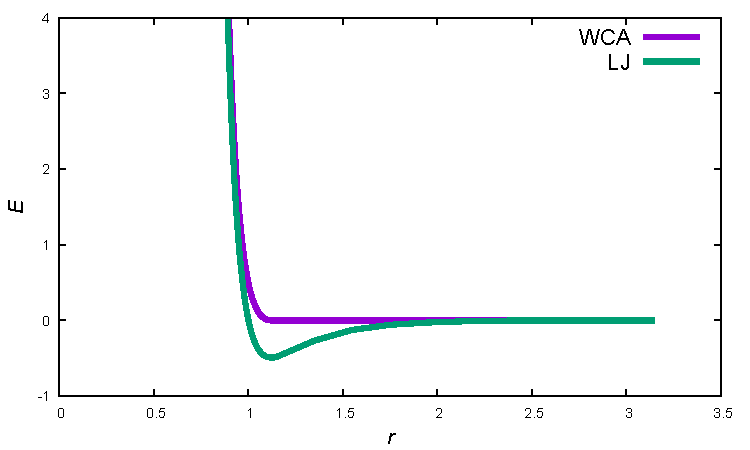
\includegraphics[width=14cm]{fig/dis-poen.pdf}
    \end{center}
    \caption{WCAとLJの原子間距離-ポテンシャルエネルギー。
    WCAポテンシャルはLJポテンシャルにカットオフ距離$r=r_c$を設けることにより、$r>r_c$でポテンシャルエネルギーが0になっている。}
    \label{fig:dis-poen}
\end{figure}

図\ref{fig:dis-poen}に示すように、WCAポテンシャルはLJポテンシャルにカットオフ距離$r=r_c$を設けることにより、
$r>r_c$でポテンシャルエネルギーが0になっている。


\section{最小二乗法}\label{principle-sec:gradient-descent}
最小二乗問題は、モデル関数とデータ点の誤差の二乗和で表される目的関数を最小化することで、パラメタ化された数学モデルをデータ点の集合に適合させるものである。今、独立変数$t$と$n$個のパラメータ$\bm{p}$のベクトルからなるモデル関数$\hat{y}(t;\bm{p})$、$m$個のデータ点$(t_i, y_i)$が存在する時、最小二乗問題は$\hat{y}(t;\bm{p})$と$m$個のデータ点$(t_i, y_i)$の間の誤差(または重み付き残差)の重み付き二乗和を最小化することに等しく、目的関数は
\large
\begin{eqnarray}
\chi^2(p) &=& \sum_{i=1}^{m}\Bigg[\frac{y(t_i)-\hat{y}(t_i;\bm{p})}{\sigma_(y_i)}\Bigg]^2 \nonumber\\
          &=& (\bm{y}-\hat{\bm{y}}(\bm{p}))^\top\bm{W}(\bm{y}-\hat{\bm{y}}(\bm{p})) \nonumber\\
          &=& \bm{y}^\top\bm{W}\bm{y}-2\bm{y}^\top\bm{W}\hat{\bm{y}}+\hat{\bm{y}}^\top\bm{W}\hat{\bm{y}} \label{eq:queue-residual-error}
\end{eqnarray}
\normalsize
と書き表せる。
ここで、$\sigma_(y_i)$はデータ$y(t_i)$の測定誤差、$\bm{W}$は重み付け行列を示す\cite{gradient-descent_gauss-newton_levenberg-marquard}。


\section{勾配降下法}\label{principle-sec:gradient-descent}
勾配降下法は、パラメタ値を下り坂方向、つまり目的関数の勾配と反対方向に更新する最小化手法である。勾配降下法は、単純な目的関数の最小化問題においては、非常によく収束することが知られている\cite{gradient-descent}。パラメタに関するカイ二乗目的関数の勾配は、
\large
\begin{eqnarray}
\frac{\partial}{\partial\bm{p}}\chi^2 &=& 2(\bm{y}-\hat{\bm{y}}(\bm{p}))^\top\bm{W}\frac{\partial}{\partial\bm{p}}(\bm{y}-\hat{\bm{y}}(\bm{p})) \nonumber\\
          &=& -2(\bm{y}-\hat{\bm{y}}(\bm{p}))^\top\bm{W}\Bigg[\frac{\partial\hat{\bm{y}}(\bm{p})}{\partial\bm{p}}\Bigg] \nonumber\\
          &=& -2(\bm{y}-\hat{\bm{y}})^\top\bm{W}\bm{J} \label{eq:gradient-of-the-chi-square-objective-function}
\end{eqnarray}
\normalsize
と書き表せる。\cite{gradient-descent_gauss-newton_levenberg-marquard}
ここで、$m×n$ヤコビアン行列$\partial\hat{\bm{y}}/{\partial\bm{p}}$は、関数の局所的な感度を表す。
また、パラメタを最急降下の方向に移動させるパラメタ更新$\bm{h}$は、
\large
\begin{eqnarray}
\bm{h} = \alpha\bm{J}^\top\bm{W}(\bm{y}-\hat{\bm{y}})
\end{eqnarray}
\normalsize
と書き表せる。
尚、正のスカラー$\alpha$は、最急降下方向のステップの長さを示す。


\section{ガウスニュートン法}\label{principle-sec:gauss-newton}


\section{Levenberg-Marquardrt法}\label{principle-sec:levenberg-marquardt}
Lebenberg-Marquardrt法は、非線形最小二乗問題を解くために1960年代初頭に開発された最適化アルゴリズムであり、様々な問題において、単純な勾配降下法や他の共役勾配法よりも大幅に優れていることが知られている\cite{levenberg-marquardt}。
Levenberg-Marquardtアルゴリズムは、勾配降下法とガウス・ニュートン法という2つの数値的最小化アルゴリズムを組み合わせたものである。勾配降下法では、最急降下方向にパラメータを更新することにより、二乗誤差の和を減少させる。ガウス・ニュートン法では、最小二乗関数は局所的に二次関数であると仮定して、二乗誤差の総和を小さくする。Levenberg-Marquardt法は、パラメータが最適値から遠い場合は勾配降下法に近い働きをし、パラメータが最適値に近い場合はガウス・ニュートン法に近い働きをする。


\chapter{手法} \label{chap:method}
\ref{method-sec:mono-component}節では、単成分LJ系における気液共存状態の実現手法を述べる。
\ref{method-sec:bi-component-azeotrope}節では、二成分LJ系における共沸現象の実現手法を述べる。
\ref{method-sec:bi-component-potential-ratio}節では、二成分LJ系におけるポテンシャルパラメタと共沸組成の関係の推定手法を述べる。
\ref{method-sec:bi-component-addition-of-3rd-component}節では、二成分LJ系への第三成分の添加手法を述べる。

\section{単成分LJ系にpおける気液共存状態の実現} \label{method-sec:mono-component}
LJ系では、ある温度、密度条件では気相と液相が相分離することが平衡状態(=気液共存状態)である事が知られている\cite{gas-liquid-equilibrium}。本節では、実際にMDシミュレーションによりこの事実を観測し、条件の近い先行研究と比較し大きな相違がないことを確認する。
初期状態として$100×50×50$の直方体の左半分に$N=78732(27×27×27×4)$個の粒子を、右半分に$N=10976(14×14×14×4)$個の粒子を面心立方(face-centered cubic, fcc)構造上に配置する。図に、原子の初期配置を示す。

% 図\ref{fig:initial-state-molecule}に、原子の初期配置を示す。
% \begin{figure}[htbp]
%     \begin{center}
%         \includegraphics[width=8cm]{}
%     \end{center}
%     \caption{原子の初期配置。
%     fcc構造上に配置されている。}
%     \label{fig:initial-state-molecule}
% \end{figure}

この初期条件の下、LJポテンシャルパラメータの${\sigma}$,\,${\varepsilon}$を共に1.0、温度$T=1.0$とし、タイムステップ0.001で500000ステップ実行のシミュレーションを行い、
粒子の密度の観測を行うことによって、気液共存状態が実現されていることを確認する。
\ref{results-sec:mono-component}節では、このシミュレーション実行時の粒子の密度の観測および、条件の近い先行研究との比較を行う。

\section{二成分LJ系における共沸現象の実現} \label{method-sec:bi-component-azeotrope}
\section{二成分LJ系におけるポテンシャルパラメタと共沸組成の関係} \label{method-sec:bi-component-potential-ratio}
\section{二成分LJ系への第三成分の添加} \label{method-sec:bi-component-addition-of-3rd-component}


\chapter{結果} \label{chap:results}
\ref{results-sec:mono-component}節では、単成分LJ系において気液共存状態を実現する。
\ref{results-sec:bi-component-azeotrope}節では、二成分LJ系において共沸現象を実現する。
\ref{results-sec:bi-component-potential-ratio}節では、二成分LJ系におけるポテンシャルパラメタと共沸組成の関係を示す。
\ref{results-sec:bi-component-addition-of-3rd-component}節では、二成分LJ系への第三成分の添加による共沸組成のずれを観測する。


\section{単成分LJ系における気液共存状態の実現} \label{results-sec:mono-component}
\ref{method-sec:mono-component}節で示したパラメタでMDシミュレーションにおいて測定された、各位置$x$\,(0.0:最小、1.0:最大において0.2〜0.8の範囲)とその密度$density$の関係を図\ref{fig:ln78732-rn10976-ld0.629856-rd0.087808-T1.0}に示す。ただし、密度$density$は、最後の5ステップを平均して取得するものとする。

\begin{figure}[htbp]
    \begin{center}
        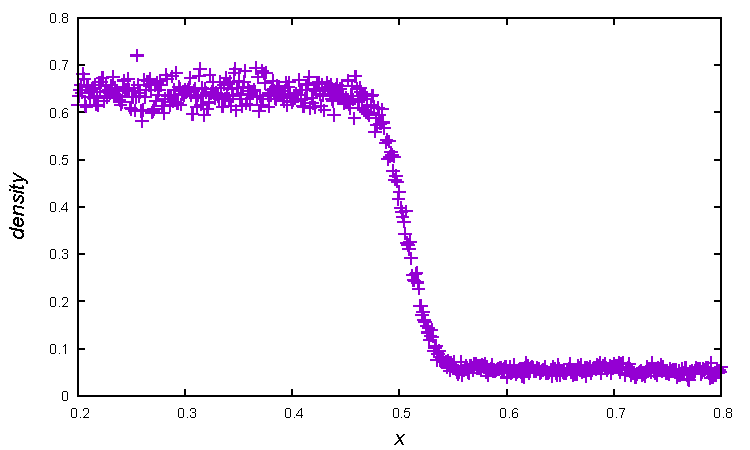
\includegraphics[width=14cm]{fig/ln78732-rn10976-ld0.629856-rd0.087808-T1.0.pdf}
    \end{center}
    \caption{単成分LJ系における密度の位置依存性}
    \label{fig:ln78732-rn10976-ld0.629856-rd0.087808-T1.0}
\end{figure}

図\ref{fig:ln78732-rn10976-ld0.629856-rd0.087808-T1.0}より、$x:0.2〜0.45$で液体状態を、$x:0.45〜0.55$で気液界面を、$x:0.55〜0.8$で気体状態をとる、気液共存状態が実現されていることが分かる。ここで、気液界面およびその近傍の密度プロファイルの関数は、次のような式で表されることが知られている\cite{gas-liquid-interface-density-profile}。
\large
\begin{eqnarray}
    \rho(x) = \frac{\rho_l+\rho_g}{2} + \frac{\rho_l-\rho_g}{2}\,tanh\Bigg(\frac{x-x_d}{2\delta_d}\Bigg) \label{eq:gas-liquid-interface-density-profile}
\end{eqnarray}
\normalsize
ここで、$\rho_l$は液相密度、$\rho_g$は気相密度、$x_d$は分割面の位置、$\delta_d$は界面厚さを示す。

式(\ref{eq:gas-liquid-interface-density-profile})により、図\ref{fig:ln78732-rn10976-ld0.629856-rd0.087808-T1.0}で得られた密度を近似したものを図\ref{fig:ln78732-rn10976-ld0.629856-rd0.087808-T1.0-fitting}に示す。

\begin{figure}[htbp]
    \begin{center}
        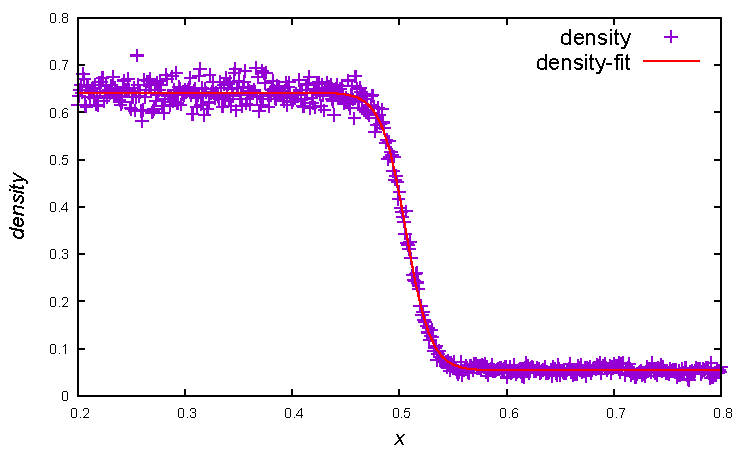
\includegraphics[width=14cm]{fig/ln78732-rn10976-ld0.629856-rd0.087808-T1.0-fitting.pdf}
    \end{center}
    \caption{単成分LJ系における密度の位置依存性及びその近似}
    \label{fig:ln78732-rn10976-ld0.629856-rd0.087808-T1.0-fitting}
\end{figure}

続いて、表\ref{table:ln78732-rn10976-ld0.629856-rd0.087808-T1.0-fitting}に、先行研究\cite{gas-liquid-equilibrium}における気液密度と、図\ref{fig:ln78732-rn10976-ld0.629856-rd0.087808-T1.0-fitting}の近似で得られた気液密度を示す。

\begin{table}[htbp]
    \begin{center}
        \caption{単成分LJ系における密度近似による気液密度値}
        \label{table:ln78732-rn10976-ld0.629856-rd0.087808-T1.0-fitting}
            \begin{tabular}{c || c | c}
                & $\rho_l$ & $\rho_g$ \\
                先行研究 & 0.5891(1) & 0.0856(2) \\
                本研究 & 0.641(1) & 0.054(1)
            \end{tabular}
    \end{center}
\end{table}

表\ref{table:ln78732-rn10976-ld0.629856-rd0.087808-T1.0-fitting}より、本研究と先行研究には誤差が存在するが、これは本研究と先行研究とでカットオフ距離近傍での原子間相互作用がわずかに違うため生じたものと考えられる。そのため、本研究で得られた結果は妥当であると判断し、表\ref{table:ln78732-rn10976-ld0.629856-rd0.087808-T1.0-fitting}で得た平衡状態における気液密度を基に、以降では初期状態で凡その気体状態、液体状態を実現した上で研究を進めることにより、平衡状態までの収束を早めた。


\section{二成分LJ系における共沸現象の実現} \label{results-sec:bi-component-azeotrope}
\section{二成分LJ系におけるポテンシャルパラメタと共沸組成の関係} \label{results-sec:bi-component-potential-ratio}
\section{二成分LJ系への第三成分の添加} \label{results-sec:bi-component-addition-of-3rd-component}

\chapter{考察および結論} \label{chap:summary}

考察は、「研究の背景」及び「目的」において提起した問題に正しく答えるようにする。得られた結果は満足すべきものだったか?不満があるならその理由はなにか?解決できそうなのか?また、「大きい理由」にも言及する。本研究によりどのような課題が見つかったかを書き、この分野における「研究の流れ」においてのような位置づけにあるかを説明した上で、今後、どのような発展の方向があるかについて書く。

\chapter*{謝辞}
まず、研究を進める上で、基礎的な部分から多くの指導をしていただいた渡辺宙志准教授には大変感謝しております。
研究のみならず、就職活動などにも気にかけ、全面的にサポートしていただき、心より御礼申し上げます。
また、同じ研究室に所属していた藤田くん、四辻くん、佐藤くんは、同期として切磋琢磨しながら研究を進めることが出来ましたこと、深く感謝致します。
最後に、研究のみならず、学生生活を様々な面でサポートしてくださった両親に深く感謝致します。

\appendix

\chapter{ソースコード}

\lstinputlisting[caption = 適当なPythonスクリプト, label = prog:sample]{src/sample.py}

\bibliographystyle{junsrt}
\bibliography{reference}

\end{document}
